\documentclass[12pt,a4paper]{article}

% ------------------------------------------------------------------ pacotes
\usepackage[T1]{fontenc}
\usepackage[utf8]{inputenc}
\usepackage[brazilian]{babel}
\usepackage{times}
\usepackage[a4paper,top=3.5cm,bottom=2.5cm,left=3cm,right=3cm]{geometry}
\usepackage{graphicx}
\usepackage{booktabs}
\usepackage{tabularx}
\usepackage{multirow}
\usepackage{float}
\renewcommand{\topfraction}{0.9}\renewcommand{\bottomfraction}{0.8}\renewcommand{\textfraction}{0.07}\renewcommand{\floatpagefraction}{0.75}
\usepackage{xcolor}
\usepackage{microtype}
\usepackage{amsmath}
\usepackage{enumitem}
\usepackage[font=small,labelfont=bf,labelsep=period]{caption}
\usepackage[square,authoryear]{natbib}
\usepackage{tikz}
\usetikzlibrary{arrows.meta,positioning,shapes.geometric}
\usepackage{xurl}
\usepackage[hidelinks]{hyperref}

\setlength{\parindent}{1.27cm}
\setlength{\parskip}{6pt}
\setlist{itemsep=2pt,topsep=4pt}
\renewcommand{\arraystretch}{1.15}
\newcolumntype{Y}{>{\raggedright\arraybackslash}X}
\newcolumntype{L}[1]{>{\raggedright\arraybackslash}p{#1}}
\bibpunct{[}{]}{;}{a}{,}{,}

% Títulos de seção no estilo SBC
\makeatletter
\renewcommand\section{\@startsection{section}{1}{\z@}{-12pt}{6pt}{\normalfont\large\bfseries}}
\renewcommand\subsection{\@startsection{subsection}{2}{\z@}{-12pt}{4pt}{\normalfont\normalsize\bfseries}}
\renewcommand\subsubsection{\@startsection{subsubsection}{3}{\z@}{-8pt}{2pt}{\normalfont\normalsize\bfseries\itshape}}
\makeatother

\newcommand{\ms}{\textit{mutation score}}
\newcommand{\MT}{\textit{Mutation Testing}}

\begin{document}

% ------------------------------------------------------------------ título
\begin{center}
  {\Large\bfseries Análise Comparativa da Efetividade de Testes Baseados em\\
  Propriedades em APIs REST Java/Spring Boot e\\
  Node.js/Express por meio de \textit{Mutation Testing}\par}
  \vspace{12pt}
  {\large Miguel Vieira\textsuperscript{1}\par}
  \vspace{6pt}
  {\small \textsuperscript{1}Bacharelado em Engenharia de Software\\
  Pontifícia Universidade Católica de Minas Gerais (PUC Minas)\\
  Belo Horizonte -- MG -- Brasil\\
  \texttt{miguel.souza.1447219@sga.pucminas.br}\par}
\end{center}

\begin{center}\textbf{Abstract}\end{center}
\vspace{-6pt}
{\small\noindent\itshape
Property-Based Testing (PBT) checks general properties over automatically generated inputs, but evidence on its effectiveness comes from single ecosystems, and mutation tools generate different mutants for the same program. This work compared the effectiveness, measured by mutation score, of equivalent PBT suites in two equivalent implementations of an event-ticketing web API, one in Java/Spring Boot (jqwik, PIT) and one in Node.js/Express (fast-check, StrykerJS). A controlled factorial experiment crossed the ecosystem, the strength of the properties (eight mostly bound-checking properties versus a suite that adds nine exact-oracle properties) and the number of tries per property (10, 100 and 1000), with 30 runs per configuration (360 runs), each tool's default mutation operators and a harmonized operator set; differences were tested with Mann-Whitney and Vargha-Delaney effect sizes. Oracle strength dominated: with 100 tries, the mutation score rose from 50.0\% to 84.1\% in Java and from 52.1\% to 95.0\% in Node.js. More tries helped only the strong suite. With default operators, Node.js scored higher in every configuration, because PIT mutates return values that state-based properties do not observe; with harmonized operators and 1000 tries, both reached 96.9\%. The ecosystem therefore matters less than how properties are written and which operators are counted.

\noindent\textbf{Keywords:} Test oracle. Test suite quality. Controlled experiment. Mutation tools.\par}

\begin{center}\textbf{Resumo}\end{center}
\vspace{-6pt}
{\small\noindent\itshape
Testes Baseados em Propriedades (PBT, do inglês \textup{Property-Based Testing}) verificam propriedades gerais sobre entradas geradas automaticamente, mas a evidência sobre sua efetividade vem de um único ecossistema, e ferramentas de mutação diferentes geram mutantes diferentes para o mesmo programa. Este trabalho comparou a efetividade, medida pelo \textup{mutation score}, de suítes PBT equivalentes em duas implementações equivalentes de uma interface de programação web de venda de ingressos, uma em Java/Spring Boot (jqwik, PIT) e outra em Node.js/Express (fast-check, StrykerJS). Um experimento controlado fatorial cruzou o ecossistema, a força das propriedades (oito propriedades que verificam sobretudo limites contra uma suíte que acrescenta nove com oráculo exato) e o número de tentativas por propriedade (10, 100 e 1000), com 30 execuções por configuração (360 execuções), os operadores de mutação padrão de cada ferramenta e um conjunto harmonizado; as diferenças foram testadas com Mann-Whitney e tamanho de efeito de Vargha-Delaney. A força do oráculo foi o fator dominante: com 100 tentativas, o \textup{mutation score} subiu de 50,0\% para 84,1\% no Java e de 52,1\% para 95,0\% no Node.js. Mais tentativas só ajudaram a suíte forte. Com os operadores padrão, o Node.js ficou acima em todas as configurações, porque o PIT muta valores de retorno que propriedades baseadas em estado não observam; com operadores harmonizados e 1000 tentativas, os dois chegaram a 96,9\%. O ecossistema pesa menos do que a forma de escrever as propriedades e os operadores considerados.

\noindent\textbf{Palavras-chave:} Oráculo de teste. Qualidade de suítes de teste. Experimento controlado. Ferramentas de mutação.\par}


\vspace{6pt}
\noindent\begin{minipage}{\textwidth}\small
\textbf{Bacharelado em Engenharia de Software -- PUC Minas}\\
Trabalho de Conclusão de Curso (TCC)\\
Orientadores de conteúdo (TCC I): Danilo Maia, João Pedro Batisteli e Leonardo Vilela\\
Orientador acadêmico (TCC I): Cleiton Tavares\\
Orientador do TCC II: Danilo Quadros Maia\\
Belo Horizonte, 30 de novembro de 2026.
\end{minipage}

\section{Introdução}

Uma suíte de testes pode executar quase todas as linhas de um sistema e, ainda assim, não perceber um comportamento incorreto. A cobertura de código mede o que foi executado, não o que foi verificado. Em APIs \textit{backend}, esse descompasso pesa porque as regras de negócio combinam limites numéricos, estados e interações entre entidades, e testes baseados em exemplos verificam apenas os cenários que o desenvolvedor lembrou de escrever.

Testes Baseados em Propriedades (PBT, do inglês \textit{Property-Based Testing}) atacam esse problema por outro ângulo: o desenvolvedor descreve uma propriedade geral do sistema e a ferramenta gera automaticamente centenas de entradas para tentar refutá-la \citep{claessen2000quickcheck}. Para medir se uma suíte de fato detecta defeitos, o \MT{} introduz pequenas alterações artificiais no código (mutantes) e verifica quantas delas fazem algum teste falhar; essa proporção é o \ms{} \citep{jia2011mutation,papadakis2019mutation}.

A evidência disponível sobre a efetividade do PBT vem quase sempre de um único ecossistema. \citet{ravi2025pbt} mediram por mutação as suítes de 40 projetos Python e mostraram que testes de propriedade encontram muito mais mutantes que testes unitários; \citet{goldstein2024pbt} e \citet{corgozinho2023pbt} estudaram como desenvolvedores escrevem propriedades, também dentro de um ecossistema. Ao mesmo tempo, ferramentas de mutação diferentes produzem conjuntos de mutantes diferentes para o mesmo programa \citep{kintis2018tools,monteiro2022tools}. Não se sabe, portanto, se as mesmas propriedades, aplicadas a implementações equivalentes em ecossistemas distintos e avaliadas pelas ferramentas de mutação de cada um, levam ao mesmo resultado. Essa é a lacuna deste trabalho.

O estudo compara Java/Spring Boot e Node.js/Express, dois dos ecossistemas mais usados para construir APIs REST, por meio de duas implementações equivalentes de uma API de gestão de eventos e reservas de ingressos. As mesmas oito propriedades de negócio foram escritas com jqwik (Java) e fast-check (Node.js) e avaliadas com PIT e StrykerJS, respectivamente.

\textbf{Questão de pesquisa geral:} suítes de testes baseadas em propriedades, derivadas das mesmas regras de negócio, têm a mesma efetividade, medida por \ms{}, quando aplicadas a implementações equivalentes de uma API REST em Java/Spring Boot e em Node.js/Express?

\textbf{Objetivo geral:} comparar, por meio do \ms{}, a efetividade de suítes PBT equivalentes nas duas implementações. Os objetivos específicos, cada um ligado às questões de pesquisa (QP) da Seção~\ref{sec:gqm}, são:

\begin{enumerate}[label=\textbf{OE\arabic*}, leftmargin=1.6cm]
  \item caracterizar as propriedades derivadas das regras de negócio e sua equivalência entre jqwik e fast-check (QP1);
  \item comparar o \ms{} das duas suítes, inclusive sob o mesmo conjunto de categorias de operadores (QP2--QP4);
  \item analisar a relação entre cobertura e \ms{} em cada ecossistema (QP5);
  \item classificar os mutantes sobreviventes segundo a regra de negócio afetada (QP6);
  \item comparar o custo de execução e o esforço de configuração das ferramentas (QP7).
\end{enumerate}

As contribuições são: (i) um experimento comparativo com 30 execuções por ecossistema e teste estatístico; (ii) a caracterização dos mutantes que sobrevivem a propriedades de invariante em cada ecossistema; e (iii) um repositório reprodutível com a especificação, as duas APIs, as suítes, os scripts de coleta e os dados brutos.

O restante do artigo está organizado assim: a Seção~2 apresenta os conceitos; a Seção~3, os trabalhos relacionados; a Seção~4, o método; a Seção~5, os resultados; a Seção~6, as ameaças à validade; e a Seção~7, as conclusões.

\section{Fundamentação Teórica}

\subsection{Testes Baseados em Propriedades}

Em PBT, o desenvolvedor escreve uma \textbf{propriedade}: uma afirmação que deve valer para todas as entradas de um domínio, como ``o total de uma reserva nunca é negativo''. Uma \textbf{invariante} é um caso particular, uma condição que toda operação deve preservar. A ferramenta usa \textbf{geradores} para produzir entradas aleatórias dentro do domínio e executa a propriedade para cada uma; quando encontra um contraexemplo, aplica \textbf{\textit{shrinking}}, reduzindo-o ao menor caso que ainda falha \citep{claessen2000quickcheck}.

As bibliotecas atuais também injetam \textbf{casos de borda} (zero, mínimo, máximo, listas vazias) entre as entradas aleatórias. O jqwik, para a JVM, roda sobre a plataforma JUnit~5 \citep{jqwik2026}; o fast-check, para JavaScript e TypeScript, roda dentro de executores como o Jest \citep{fastcheck2026}. Ambos geram valores aleatórios com semente nova a cada execução, por padrão.

A qualidade de uma suíte PBT depende de duas coisas. A primeira é o \textbf{oráculo}, isto é, o que cada propriedade verifica. Uma propriedade que só checa limites (``$0 \le \text{desconto} \le \text{subtotal}$'') aceita qualquer cálculo que respeite esses limites; uma que compara o sistema com um \textbf{modelo de referência} verifica valores exatos. A segunda é a \textbf{amostra de entradas}: o número de tentativas por propriedade e a forma como o gerador distribui os valores. Um defeito que só aparece em um valor exato, como o último dia de validade de um cupom, só é encontrado se o gerador produzir esse valor. O experimento deste trabalho varia os dois aspectos.

\subsection{\textit{Mutation Testing}}

O \MT{} aplica \textbf{operadores de mutação} ao programa, cada um gerando uma versão com uma pequena alteração: trocar \texttt{<} por \texttt{<=}, \texttt{+} por \texttt{-}, remover uma chamada, devolver \texttt{null}. A suíte é executada contra cada mutante \citep{jia2011mutation}. O mutante é \textbf{morto} quando algum teste falha, \textbf{sobrevivente} quando todos passam e \textbf{sem cobertura} quando nenhum teste executa o trecho alterado. Mutantes que estouram o tempo limite contam como detectados. O \ms{} é:

\begin{equation}
MS = \frac{K + T}{K + T + S + N} \times 100\%
\label{eq:ms}
\end{equation}

\noindent em que $K$, $T$, $S$ e $N$ são os mutantes mortos, com \textit{timeout}, sobreviventes e sem cobertura. Mutantes que não compilam ou quebram a execução ficam de fora, como fazem PIT e StrykerJS.

Um \textbf{mutante equivalente} altera o código sem alterar o comportamento observável e, por isso, nunca pode ser morto. Identificá-los exige análise manual \citep{papadakis2019mutation}. Além disso, o conjunto de operadores varia entre ferramentas: o PIT muta \textit{bytecode} Java \citep{coles2016pit} e seu conjunto padrão é mais restrito que o recomendado na literatura \citep{laurent2017pit}; o StrykerJS muta a árvore sintática de JavaScript e inclui operadores sem equivalente no PIT, como a troca de literais de texto \citep{stryker2026}. Comparar ecossistemas exige, portanto, controlar também o conjunto de operadores, restringindo a comparação às transformações que as duas ferramentas aplicam da mesma forma.

\section{Trabalhos Relacionados}

Foram selecionados seis estudos empíricos de Engenharia de Software que avaliam PBT, a relação entre cobertura e \MT{} ou ferramentas de mutação; quatro deles foram publicados entre 2023 e 2025. Para cada um, apresentam-se objetivo e método, os resultados relevantes e a relação com este trabalho. A Tabela~\ref{tab:relacionados} resume o posicionamento.

\textbf{\citet{ravi2025pbt}} avaliaram a efetividade de PBT em Python. Analisaram 426 programas que usam a biblioteca Hypothesis, definiram 12 categorias de propriedade e aplicaram \MT{} às suítes de 40 projetos. Cada teste de propriedade encontrou, em média, cerca de 50 vezes mais mutações que um teste unitário; testes que verificam exceções, pertinência e tipos foram os mais efetivos; e 76\% das mutações encontradas apareceram nas primeiras 20 entradas geradas. É o trabalho mais próximo deste. Aqui, a mesma pergunta é feita em dois ecossistemas, com propriedades controladas, e o efeito do número de entradas é medido diretamente (10, 100 e 1000 tentativas).

\textbf{\citet{goldstein2024pbt}} investigaram como o PBT é usado na prática por meio de 30 entrevistas semiestruturadas na Jane Street, empresa que usa PBT em OCaml, com análise temática. Os participantes concentraram o uso em poucos padrões de alto retorno, como comparação com um modelo de referência e propriedades de ida e volta, e relataram dificuldade em escrever geradores e em avaliar a efetividade das suítes. Este trabalho responde a essa dificuldade de forma quantitativa: mede, por mutação, quanto propriedades com modelo de referência detectam a mais que propriedades de limite.

\textbf{\citet{corgozinho2023pbt}} caracterizaram como desenvolvedores implementam propriedades, classificando 86 testes de propriedade de 30 repositórios Python. Propriedades de ida e volta (37,2\%) e de oráculo (33,7\%) somaram 70,9\% dos testes. As categorias catalogadas por esse estudo orientaram a escolha das propriedades da suíte fraca deste trabalho, cuja efetividade é agora medida.

\textbf{\citet{jain2023gap}} propuseram a ``lacuna de oráculo'', a diferença entre cobertura e \ms{}, e a estudaram em 45 projetos Java, em arquivos com asserções removidas e em código de criptomoedas. Sobre o código coberto, cobertura e \ms{} tiveram correlação fraca (0,21), e remover asserções ampliou a lacuna. A QP5 deste trabalho mede essa lacuna em PBT e mostra como ela se fecha quando o oráculo das propriedades fica mais forte.

\textbf{\citet{kintis2018tools}} compararam quatro ferramentas de mutação para Java (PIT, muJava, Major e PITRV) com análise manual dos mutantes e com defeitos reais. A efetividade variou muito entre as ferramentas, e nenhuma subsumiu as demais. \textbf{\citet{monteiro2022tools}} compararam PIT e Major: o PIT gerou significativamente mais mutantes, com desempenho um pouco melhor, mas o Major superou o PIT quando os mutantes possivelmente equivalentes foram excluídos. Esses resultados motivam o recorte harmonizado de operadores deste trabalho, que estende a comparação de ferramentas ao par PIT/StrykerJS, entre linguagens.

\begin{table}[!htbp]
\centering
\caption{Posicionamento dos trabalhos relacionados.}
\label{tab:relacionados}
\small
\begin{tabularx}{\textwidth}{@{}L{3.4cm} Y c c c@{}}
\toprule
Trabalho & Método e linguagem & PBT & Mutação & Compara ecossistemas \\
\midrule
\citet{ravi2025pbt} & Mineração e mutação, Python & sim & sim & não \\
\citet{goldstein2024pbt} & Entrevistas, OCaml & sim & não & não \\
\citet{corgozinho2023pbt} & Mineração, Python & sim & não & não \\
\citet{jain2023gap} & Cobertura $\times$ mutação, Java & não & sim & não \\
\citet{kintis2018tools}; \citet{monteiro2022tools} & Comparação de ferramentas, Java & não & sim & não \\
\textbf{Este trabalho} & Experimento, Java e Node.js & sim & sim & sim \\
\bottomrule
\end{tabularx}
\end{table}

\section{Materiais e Métodos}

\subsection{Tipo de pesquisa}

Trata-se de um experimento controlado comparativo, com análise quantitativa (\ms{}, contagens de mutantes, cobertura e tempo, em 30 execuções por ecossistema) e qualitativa (classificação manual dos mutantes sobreviventes e registro do esforço de configuração). O fator estudado é o ecossistema, com dois níveis: Java/Spring Boot com jqwik e PIT, e Node.js/Express com fast-check e StrykerJS. Como cada ecossistema usa sua própria ferramenta de mutação, o fator é o par ``linguagem + ferramentas'', e não a linguagem isolada; essa escolha é discutida na Seção~6.

\subsection{Objetivos, questões e métricas (GQM)}
\label{sec:gqm}

O estudo segue o modelo \textit{Goal-Question-Metric} \citep{basili1994gqm}. O objetivo é: \textit{analisar} suítes de testes baseadas em propriedades \textit{com o propósito de} compará-las \textit{com respeito à} efetividade medida por \ms{} \textit{do ponto de vista} do desenvolvedor \textit{no contexto de} duas implementações equivalentes de uma API REST em Java/Spring Boot e Node.js/Express. A Tabela~\ref{tab:gqm} desdobra esse objetivo em questões e métricas; a Tabela~\ref{tab:metricas} define cada métrica.

\begin{table}[!htbp]
\centering
\caption{Desdobramento GQM: objetivos específicos, questões de pesquisa e métricas.}
\label{tab:gqm}
\small
\begin{tabularx}{\textwidth}{@{}l Y l@{}}
\toprule
OE & Questão de pesquisa & Métricas \\
\midrule
OE1 & QP1: Quais regras de negócio puderam ser expressas como propriedades equivalentes nos dois ecossistemas? & M1, M2, M3 \\
OE2 & QP2: Qual o \ms{} de cada suíte? & M4, M5 \\
OE2 & QP3: A diferença de \ms{} entre ecossistemas é estatisticamente significativa, e de que tamanho? & M6 \\
OE2 & QP4: A diferença se mantém quando só as categorias de operadores comuns às duas ferramentas são consideradas? & M7 \\
OE3 & QP5: Os mutantes cobertos pela suíte são também detectados por ela? & M8, M9 \\
OE4 & QP6: Quais regras e propriedades concentram mutantes sobreviventes, e por quê? & M10, M11 \\
OE5 & QP7: Qual ecossistema exige mais tempo de execução e esforço de configuração? & M12, M13, M14 \\
\bottomrule
\end{tabularx}
\end{table}

\begin{table}[!htbp]
\centering
\caption{Métricas: definição, forma de coleta e questão atendida.}
\label{tab:metricas}
\small
\begin{tabularx}{\textwidth}{@{}l L{2.9cm} Y L{2.6cm} l@{}}
\toprule
Id & Métrica & Definição / fórmula & Fonte & QP \\
\midrule
M1 & Regras cobertas & Regras R1--R20 verificadas por ao menos uma propriedade / 20 & \texttt{SPEC.md} & QP1 \\
M2 & Propriedades equivalentes & Propriedades de P1--P8 implementadas nos dois ecossistemas com o mesmo enunciado e os mesmos geradores & código & QP1 \\
M3 & Tamanho das suítes & Linhas de código não vazias e não comentário de propriedades e geradores & código & QP1, QP7 \\
M4 & Contagens de mutantes & Gerados, mortos, \textit{timeout}, sobreviventes, sem cobertura e erros & PIT XML, Stryker JSON & QP2 \\
M5 & \textit{Mutation score} & Equação~\ref{eq:ms}, sobre todos os mutantes válidos & idem & QP2 \\
M6 & Diferença de \ms{} & Mann-Whitney U, $p$-valor e $\hat{A}_{12}$ sobre os 30 valores por ecossistema & \texttt{runs.csv} & QP3 \\
M7 & \textit{Score} por categoria & Equação~\ref{eq:ms} restrita às categorias de operadores comuns (Tabela~\ref{tab:categorias}) & \texttt{mutants.csv} & QP4 \\
M8 & Cobertura & Linhas e ramos do domínio cobertos pela suíte de propriedades & JaCoCo, Istanbul & QP5 \\
M9 & Cobertura de mutantes & Mutantes não classificados como ``sem cobertura'' / mutantes válidos, por módulo & \texttt{mutants.csv} & QP5 \\
M10 & Sobreviventes por recorte & Sobreviventes por módulo, categoria, e mortes por propriedade & \texttt{mutants.csv} & QP6 \\
M11 & Classe do sobrevivente & Classificação manual: equivalente, propriedade fraca ou regra sem propriedade & análise manual & QP6 \\
M12 & Tempo & Tempo de parede da suíte e da análise de mutação, por execução & \texttt{runs.csv} & QP7 \\
M13 & Mutantes por execução & Média de mutantes válidos gerados por execução & \texttt{runs.csv} & QP7 \\
M14 & Esforço de configuração & Arquivos de configuração, dependências e problemas registrados até a primeira execução & diário & QP7 \\
\bottomrule
\end{tabularx}
\end{table}

\subsection{Aplicação de referência}

A aplicação é uma API REST de gestão de eventos e reservas de ingressos, inspirada no domínio de plataformas como a Ticketmaster Discovery API \citep{ticketmaster2026}. A API externa não é o objeto do experimento, porque o \MT{} exige acesso ao código. As regras foram fixadas em uma especificação única (\texttt{SPEC.md}), escrita antes das implementações, com 20 regras numeradas. A Tabela~\ref{tab:regras} as resume por módulo.

\begin{table}[!htbp]
\centering
\caption{Módulos e regras de negócio da aplicação de referência.}
\label{tab:regras}
\small
\begin{tabularx}{\textwidth}{@{}l l Y@{}}
\toprule
Módulo & Regras & Conteúdo \\
\midrule
Eventos & R1, R2 & Capacidade $> 0$ e nome não vazio; só eventos \texttt{ATIVO} aceitam reservas, itens e confirmações. \\
Lotes & R3--R5 & Preço $\ge 0$ e quantidade $> 0$; soma das quantidades dos lotes $\le$ capacidade do evento; $0 \le$ disponível $\le$ total. \\
Reservas & R6--R8 & Reserva nasce \texttt{CRIADA}; itens só em reserva \texttt{CRIADA}, com quantidade $> 0$ e lote do mesmo evento; subtotal $= \sum$ preço $\times$ quantidade. \\
Cupons & R9--R13 & Percentual em [1, 100] ou fixo $> 0$; desconto $= \lfloor$subtotal $\times$ \%$/100\rfloor$ ou valor fixo, limitado ao teto; desconto zero se o cupom não existe, expirou ou o subtotal está abaixo do mínimo; $0 \le$ desconto $\le$ subtotal. \\
Disponibilidade & R14--R17 & Confirmar exige itens e evento ativo; verifica todos os lotes antes de baixar qualquer um (tudo ou nada); cancelar ou expirar reserva confirmada devolve as quantidades. \\
Status & R18--R20 & Transições da Figura~\ref{fig:estados}; estados finais não mudam; entidade inexistente gera erro de ``não encontrado''. \\
\bottomrule
\end{tabularx}
\end{table}

\begin{figure}[!htbp]
\centering
\begin{tikzpicture}[
  estado/.style={draw, rounded corners=4pt, minimum width=2.3cm, minimum height=0.8cm, font=\small},
  final/.style={estado, double},
  seta/.style={-{Stealth[length=2mm]}, thick},
  rot/.style={font=\scriptsize, inner sep=2pt}]
  \node[estado] (criada) at (0,0) {CRIADA};
  \node[estado] (confirmada) at (5,0) {CONFIRMADA};
  \node[final] (paga) at (9.2,0) {PAGA};
  \node[final] (cancelada) at (2.5,-1.6) {CANCELADA};
  \node[final] (expirada) at (2.5,-3.0) {EXPIRADA};
  \draw[seta] (criada) -- node[rot, above] {confirmar} (confirmada);
  \draw[seta] (confirmada) -- node[rot, above] {pagar} (paga);
  \draw[seta] (criada.south east) -- node[rot, above right, pos=0.4] {cancelar} (cancelada.north west);
  \draw[seta] (confirmada.south west) -- node[rot, above left, pos=0.4] {cancelar$^{*}$} (cancelada.north east);
  \draw[seta] (criada.south) |- node[rot, left, pos=0.4] {expirar} (expirada.west);
  \draw[seta] (confirmada.south) |- node[rot, right, pos=0.4] {expirar$^{*}$} (expirada.east);
\end{tikzpicture}
\caption{Transições de status da reserva (R18). Estados com borda dupla são finais (R19). $^{*}$Devolve a disponibilidade dos lotes (R17).}
\label{fig:estados}
\end{figure}

\subsection{Implementações e ferramentas}

As duas implementações expõem as mesmas 14 rotas REST e delegam toda a regra a um serviço de domínio com persistência em memória. A Tabela~\ref{tab:ferramentas} lista as versões. O código, a especificação, os scripts e os dados brutos estão no repositório do trabalho\footnote{\url{https://github.com/migueltico2/tcc-pbt-mutation}}.

\begin{table}[!htbp]
\centering
\caption{Ferramentas e versões usadas no experimento.}
\label{tab:ferramentas}
\small
\begin{tabularx}{\textwidth}{@{}l Y Y@{}}
\toprule
Papel & Java & Node.js \\
\midrule
Plataforma & Java 17 (\texttt{--release 17}, JDK 21) & Node.js 22.22 \\
Camada REST & Spring Boot 3.3.5 & Express 5.3 \\
Executor de testes & JUnit Platform 1.9 & Jest 30.5 \\
PBT & jqwik 1.7.4 & fast-check 4.10.2 \\
Mutação & PIT 1.18.2 + pitest-junit5-plugin 1.2.3, mutadores \texttt{DEFAULTS} & StrykerJS 10.0 + jest-runner, mutadores padrão \\
Cobertura & JaCoCo 0.8.12 & Istanbul (via Jest) \\
\bottomrule
\end{tabularx}
\end{table}

A equivalência funcional foi verificada por 11 cenários de exemplo compartilhados (\texttt{shared/casos-exemplo.json}), com 125 passos, dos quais 28 esperam um código de erro específico. O mesmo arquivo é lido por um executor em cada ecossistema, e os 11 cenários passam nas duas implementações. Esses testes de exemplo não entram na análise de mutação.

\subsection{Propriedades}

As oito propriedades previstas no TCC~I foram implementadas nos dois ecossistemas com o mesmo enunciado, os mesmos geradores (mesmas faixas de valores) e 100 tentativas por propriedade (Tabela~\ref{tab:propriedades}). Os geradores produzem de 1 a 4 lotes (preço de 0 a 100\,000 centavos, quantidade de 1 a 50), de 1 a 5 itens (quantidade de 1 a 10) e cupons percentuais ou fixos com mínimo, teto opcional (ausente em 25\% dos casos) e validade de $\pm 30$ dias.

\begin{table}[!htbp]
\centering
\caption{Propriedades implementadas, regras verificadas e tipo de oráculo.}
\label{tab:propriedades}
\small
\begin{tabularx}{\textwidth}{@{}L{3.3cm} Y l l@{}}
\toprule
Propriedade & Enunciado & Regras & Oráculo \\
\midrule
P1 Total não negativo & Para qualquer reserva e cupom (válido, inexistente ou ausente), total $\ge 0$ & R8, R11--R13 & limite \\
P2 Desconto limitado & $0 \le$ desconto $\le$ subtotal e total $=$ subtotal $-$ desconto & R11, R13 & limite \\
P3 Comutatividade & Permutar os itens não altera o subtotal & R8 & metamórfico \\
P4 Cupom inválido neutro & Cupom inexistente, expirado ou com mínimo acima do subtotal não altera o total & R12 & neutralidade \\
P5 Disponibilidade não negativa & Após confirmações aceitas ou recusadas, $0 \le$ disponível $\le$ total & R5, R15 & limite \\
P6 Redução correta & Confirmação aceita reduz exatamente o pedido; recusada não altera lotes & R15, R16 & valor exato \\
P7 Cancelamento restaura & Confirmar e cancelar (ou expirar) devolve a disponibilidade inicial & R17 & ida e volta \\
P8 Transições válidas & Sequências de 1 a 8 operações seguem o modelo da Figura~\ref{fig:estados} ou são recusadas sem mudar o status & R18, R19 & modelo \\
\bottomrule
\end{tabularx}
\end{table}

\subsection{Decisões de projeto do experimento}

Para tornar a comparação justa e viável, foram tomadas as decisões abaixo, todas registradas no repositório:

\begin{itemize}
  \item \textbf{Mutação só no domínio.} PIT e StrykerJS mutam apenas a camada de domínio (pacote \texttt{domain} e pasta \texttt{src/domain}); controladores e configuração do framework não contêm regra de negócio e só gerariam ruído.
  \item \textbf{Propriedades chamam o domínio diretamente}, não via HTTP, para que o tempo medido não inclua o custo de cada servidor web.
  \item \textbf{Dinheiro em centavos inteiros} nos dois lados, evitando divergências de ponto flutuante que não são do ecossistema.
  \item \textbf{Só a suíte de propriedades} é usada na mutação e na cobertura; os testes de exemplo ficam de fora.
  \item \textbf{Configurações equivalentes:} 100 tentativas, geração aleatória e semente nova a cada execução nos dois lados. No jqwik, o reaproveitamento da semente que falhou na execução anterior foi desligado, para que um mutante não influencie o próximo.
  \item \textbf{Matriz completa de mortes:} o PIT registra todos os testes que matam cada mutante (\textit{full mutation matrix}) e o StrykerJS foi configurado para não parar no primeiro teste que falha (\texttt{disableBail}), o que permite atribuir cada morte a uma ou mais propriedades.
  \item \textbf{Ferramentas como usadas na prática:} cada ferramenta de mutação roda com seu conjunto padrão de operadores. A comparação justa entre operadores é feita depois, por categorias (Tabela~\ref{tab:categorias}).
\end{itemize}

\begin{table}[!htbp]
\centering
\caption{Categorias de operadores usadas para comparar as ferramentas. As cinco primeiras existem nas duas. $^{\dagger}$O grupo \texttt{DEFAULTS} do PIT 1.18 não inclui \texttt{NegateConditionals}; por isso, no Java, a categoria contém apenas mutantes de limite, enquanto o \texttt{EqualityOperator} do StrykerJS também nega comparações.}
\label{tab:categorias}
\small
\begin{tabularx}{\textwidth}{@{}l Y Y@{}}
\toprule
Categoria & PIT (\texttt{DEFAULTS}) & StrykerJS \\
\midrule
Aritmético & \texttt{Math}, \texttt{InvertNegs} & \texttt{ArithmeticOperator}, \texttt{AssignmentOperator}, \texttt{UnaryOperator} \\
Relacional & \texttt{ConditionalsBoundary}$^{\dagger}$ & \texttt{EqualityOperator} \\
Condicional/lógico & \texttt{RemoveConditional\_*} & \texttt{ConditionalExpression}, \texttt{LogicalOperator} \\
Remoção de instrução & \texttt{VoidMethodCall} & \texttt{BlockStatement}, \texttt{CallExpression} \\
Incremento & \texttt{Increments} & \texttt{UpdateOperator} \\
\midrule
Valor de retorno & \texttt{EmptyObject}, \texttt{Null}, \texttt{Primitive}, \texttt{True}/\texttt{FalseReturnVals} & --- \\
Literal & --- & \texttt{StringLiteral}, \texttt{BooleanLiteral}, \texttt{ObjectLiteral}, \texttt{ArrayDeclaration} \\
Chamada de método & --- & \texttt{MethodExpression}, \texttt{OptionalChaining} \\
\bottomrule
\end{tabularx}
\end{table}

\subsection{Procedimento e ambiente de execução}

O experimento seguiu seis etapas (Figura~\ref{fig:procedimento}). Cada uma das 30 execuções por ecossistema roda a suíte de propriedades com cobertura e, em seguida, a análise de mutação completa, gravando os relatórios brutos. Um script consolida os relatórios em duas tabelas: uma linha por execução (\texttt{runs.csv}) e uma linha por mutante por execução (\texttt{mutants.csv}). As execuções foram sequenciais (primeiro as 30 do Java, depois as 30 do Node.js), na mesma máquina virtual: 2 vCPUs Intel Xeon de 2,1~GHz, 7~GB de RAM, Ubuntu 24.04, com duas \textit{threads} de mutação em cada ferramenta.

\begin{figure}[!htbp]
\centering
\begin{tikzpicture}[
  etapa/.style={draw, rounded corners=4pt, align=center, font=\scriptsize, minimum height=1.0cm, text width=1.85cm},
  seta/.style={-{Stealth[length=1.8mm]}, thick}, node distance=0.3cm]
  \node[etapa] (e1) {1. Especificação (\texttt{SPEC.md})};
  \node[etapa, right=of e1] (e2) {2. Duas APIs + casos compartilhados};
  \node[etapa, right=of e2] (e3) {3. P1--P8 em jqwik e fast-check};
  \node[etapa, right=of e3] (e4) {4. 30 execuções: cobertura + mutação};
  \node[etapa, right=of e4] (e5) {5. Consolidação (CSV)};
  \node[etapa, right=of e5] (e6) {6. Análise e testes estatísticos};
  \foreach \a/\b in {e1/e2,e2/e3,e3/e4,e4/e5,e5/e6} \draw[seta] (\a) -- (\b);
\end{tikzpicture}
\caption{Etapas do procedimento experimental.}
\label{fig:procedimento}
\end{figure}

O ambiente de execução não tinha acesso ao repositório Maven Central. Por isso, jqwik 1.7.4 e PIT 1.18.2 foram compilados a partir do código-fonte das versões publicadas, e a suíte Java foi executada pelo JUnit Platform Console, com o PIT acionado pela mesma API que o \textit{plugin} Maven usa. O \texttt{pom.xml} do repositório declara as mesmas versões, de modo que o experimento pode ser repetido com \texttt{mvn}. O esforço de configuração (M14) considera os dois caminhos.

\subsection{Análise dos dados}

O \ms{} de cada execução forma uma amostra de 30 valores por ecossistema. Como o PBT é aleatório e não há garantia de normalidade, a diferença entre ecossistemas foi testada com Mann-Whitney U bilateral \citep{mann1947test} a $\alpha = 0{,}05$, e o tamanho do efeito foi medido pela estatística $\hat{A}_{12}$ de Vargha-Delaney \citep{vargha2000a12}, seguindo a recomendação de \citet{arcuri2011guide} para algoritmos aleatórios em Engenharia de Software. $\hat{A}_{12}$ é a probabilidade de uma execução Java ter valor maior que uma Node.js; $0{,}5$ indica nenhuma diferença, e as faixas de magnitude são as de \citet{vargha2000a12}. O teste de Shapiro-Wilk foi usado apenas para descrever a distribuição. As hipóteses são:

\begin{itemize}
  \item $H_{0,1}$: o \ms{} das suítes PBT não difere entre Java e Node.js; $H_{1,1}$: difere.
  \item $H_{0,2}$: o tempo da análise de mutação não difere entre os ecossistemas; $H_{1,2}$: difere.
\end{itemize}

Os mutantes sobreviventes foram agrupados por localização e operador e classificados manualmente em três classes: \textbf{equivalente} (nenhuma entrada distingue o mutante do original), \textbf{propriedade fraca} (a regra é exercitada por uma propriedade, mas o oráculo não observa a diferença) e \textbf{regra sem propriedade} (a regra afetada não é verificada por nenhuma de P1--P8).

\section{Resultados e Discussão}

\subsection{Sumarização dos resultados}

Foram realizadas \totalExecucoes{} execuções completas, com \totalAvaliacoes{} avaliações de mutantes (excluídos os erros de execução). Por execução, o PIT gerou \gerJavaFracaCem{} mutantes com seu conjunto padrão e o StrykerJS, \gerNodeFracaCem; no recorte harmonizado, os dois conjuntos ficaram quase do mesmo tamanho (\gerhJavaFracaCem{} e \gerhNodeFracaCem), com a mesma distribuição por classe. A Tabela~\ref{tab:resumo} resume cada configuração, e a Figura~\ref{fig:tentativas} mostra o \ms{} em função do número de tentativas.

\begin{table}[!htbp]
\centering
\caption{\textit{Mutation score} (mediana e intervalo interquartil das 30 execuções) com operadores padrão e harmonizados, cobertura de linhas e ramos e mutantes instáveis (M6), por configuração.}
\label{tab:resumo}
\small\setlength{\tabcolsep}{4pt}
\begin{tabular*}{\textwidth}{@{\extracolsep{\fill}}l l r r c r c r@{}}
\toprule
 & & & \multicolumn{2}{c}{\textit{Mutation score} padrão (\%)} & Harmon. & Cobertura (\%) & \\
Ecossistema & Suíte & Tent. & Mediana & IQR & (\%) & linhas / ramos & Instáveis \\
\midrule
Java & fraca & 10 & \msJavaFracaDez & \msqJavaFracaDez & \mshJavaFracaDez & \coblJavaFracaDez{} / \cobrJavaFracaDez & \instJavaFracaDez \\
 &  & 100 & \msJavaFracaCem & \msqJavaFracaCem & \mshJavaFracaCem & \coblJavaFracaCem{} / \cobrJavaFracaCem & \instJavaFracaCem \\
 &  & 1000 & \msJavaFracaMil & \msqJavaFracaMil & \mshJavaFracaMil & \coblJavaFracaMil{} / \cobrJavaFracaMil & \instJavaFracaMil \\
 & forte & 10 & \msJavaForteDez & \msqJavaForteDez & \mshJavaForteDez & \coblJavaForteDez{} / \cobrJavaForteDez & \instJavaForteDez \\
 &  & 100 & \msJavaForteCem & \msqJavaForteCem & \mshJavaForteCem & \coblJavaForteCem{} / \cobrJavaForteCem & \instJavaForteCem \\
 &  & 1000 & \msJavaForteMil & \msqJavaForteMil & \mshJavaForteMil & \coblJavaForteMil{} / \cobrJavaForteMil & \instJavaForteMil \\
\midrule
Node.js & fraca & 10 & \msNodeFracaDez & \msqNodeFracaDez & \mshNodeFracaDez & \coblNodeFracaDez{} / \cobrNodeFracaDez & \instNodeFracaDez \\
 &  & 100 & \msNodeFracaCem & \msqNodeFracaCem & \mshNodeFracaCem & \coblNodeFracaCem{} / \cobrNodeFracaCem & \instNodeFracaCem \\
 &  & 1000 & \msNodeFracaMil & \msqNodeFracaMil & \mshNodeFracaMil & \coblNodeFracaMil{} / \cobrNodeFracaMil & \instNodeFracaMil \\
 & forte & 10 & \msNodeForteDez & \msqNodeForteDez & \mshNodeForteDez & \coblNodeForteDez{} / \cobrNodeForteDez & \instNodeForteDez \\
 &  & 100 & \msNodeForteCem & \msqNodeForteCem & \mshNodeForteCem & \coblNodeForteCem{} / \cobrNodeForteCem & \instNodeForteCem \\
 &  & 1000 & \msNodeForteMil & \msqNodeForteMil & \mshNodeForteMil & \coblNodeForteMil{} / \cobrNodeForteMil & \instNodeForteMil \\
\midrule
Java & \multicolumn{2}{l}{11 exemplos} & \baseJava & --- & \basehJava & --- & --- \\
Node.js & \multicolumn{2}{l}{11 exemplos} & \baseNode & --- & \basehNode & --- & --- \\
\bottomrule
\end{tabular*}
\end{table}

\begin{figure}[!htbp]
\centering
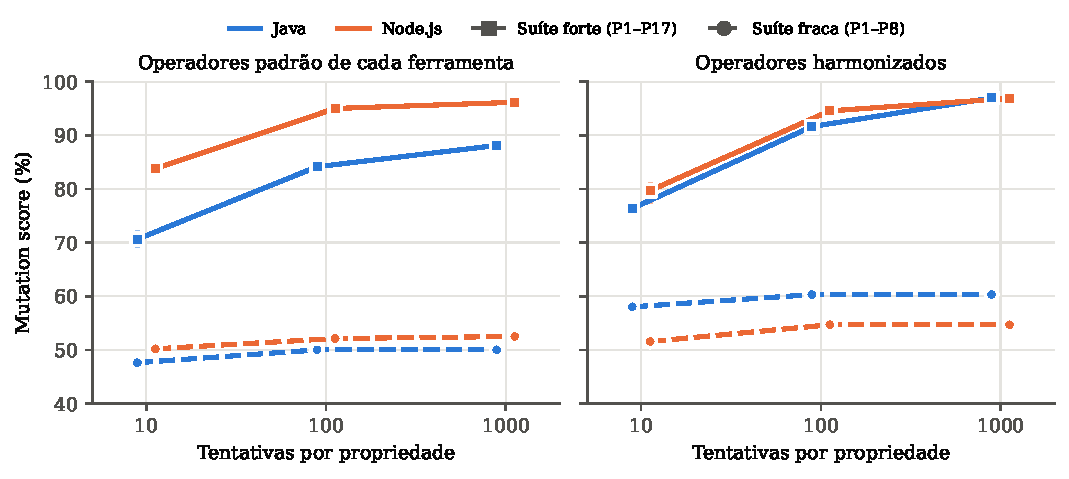
\includegraphics[width=\textwidth]{figuras/fig5_1_score_tentativas.pdf}
\caption{\textit{Mutation score} por número de tentativas, suíte e ecossistema: mediana (marcador) e intervalo interquartil (barra vertical) das 30 execuções. Linhas cheias: suíte forte; tracejadas: suíte fraca.}
\label{fig:tentativas}
\end{figure}

A configuração da versão anterior deste trabalho (suíte fraca, 100 tentativas) foi reproduzida: \msJavaFracaCem\% no Java e \msNodeFracaCem\% no Node.js. As figuras complementares (por classe de mutação, por módulo, por propriedade e de tempo) estão no Apêndice~\ref{ap:figuras}.

\subsection{Discussão dos resultados}

\textbf{QP1 -- Quais regras puderam ser expressas como propriedades equivalentes, e com que oráculo?} Todas. As 17 propriedades foram implementadas nos dois ecossistemas com o mesmo enunciado, as mesmas faixas de geração e o mesmo número de tentativas (M2 = 17/17). A suíte fraca verifica 10 das 20 regras (M1 = 50\%) e nenhuma de suas propriedades confere o valor do preço; a suíte forte verifica as 20 (M1 = 100\%). O tamanho foi equivalente: 336 linhas no Java e 293 no Node.js para a suíte fraca, mais 513 e 446 para as propriedades novas. O jqwik exigiu tipos explícitos para cada dado gerado, enquanto o fast-check compõe geradores em linha; nenhuma propriedade precisou ser adaptada.

\textbf{QP2 -- Qual o \ms{} de cada suíte, e quanto a força do oráculo o altera?} Com 100 tentativas, a suíte fraca detectou \msJavaFracaCem\% (Java) e \msNodeFracaCem\% (Node.js) dos mutantes, e a suíte forte, \msJavaForteCem\% e \msNodeForteCem\%. A suíte forte foi superior em todas as comparações entre execuções ($\hat{A}_{12} = 1$, $p < 0{,}001$ em todas as combinações), com ganho de 23 a 44 pontos. Os 11 cenários de exemplo detectaram \baseJava\% e \baseNode\%, muito acima da suíte fraca, porque conferem valores exatos, inclusive o objeto devolvido por cada operação. Quando as propriedades também conferem valores exatos, elas alcançam os exemplos: no recorte harmonizado, a suíte forte com 1000 tentativas chegou a \mshJavaForteMil\% e \mshNodeForteMil\%, contra \basehJava\% e \basehNode\% dos exemplos.

\textbf{QP3 -- O número de tentativas altera o \ms{}?} Só com propriedades fortes. Na suíte forte, ir de 10 para 100 tentativas elevou o \ms{} de \msJavaForteDez\% para \msJavaForteCem\% no Java e de \msNodeForteDez\% para \msNodeForteCem\% no Node.js; de 100 para 1000, o ganho foi menor (\msJavaForteMil\% e \msNodeForteMil\%). Na suíte fraca, a variação ficou abaixo de 3 pontos, e no Java as 60 execuções com 100 e 1000 tentativas deram o mesmo resultado. Os mutantes que dependem de um valor exato de limite alternam entre detectados e sobreviventes quando há poucas tentativas: na suíte forte, \instJavaForteDez{} (Java) e \instNodeForteDez{} (Node.js) mudaram de resultado entre execuções com 10 tentativas, contra \instJavaForteMil{} e \instNodeForteMil{} com 1000. Mais entradas só ajudam quando o oráculo reconhece o defeito que elas revelam, o que complementa a observação de \citet{ravi2025pbt} de que a maioria das mutações aparece nas primeiras entradas.

\textbf{QP4 -- O \ms{} difere entre os ecossistemas?} Depende dos operadores (Tabela~\ref{tab:testes}). Com os operadores padrão, $H_0$ foi rejeitada em todas as configurações, sempre com o Node.js acima ($\hat{A}_{12} \le 0{,}01$). A diferença vem da ferramenta: o PIT gera mutantes de valor de retorno (por exemplo, devolver \texttt{null} no lugar da reserva atualizada) que as propriedades não observam, porque consultam o estado depois da operação, e o StrykerJS não tem esse operador. No recorte harmonizado, a relação se inverte na suíte fraca (\mshJavaFracaCem\% no Java contra \mshNodeFracaCem\% no Node.js) e, na suíte forte com 1000 tentativas, $H_0$ não foi rejeitada (\mshJavaForteMil\% nos dois, \pEcoForteMilHarm). Com o mutante distinto como unidade e 100 tentativas, nenhuma diferença harmonizada foi significativa (suíte fraca: $\chi^2 = $ \chiFraca, \pchiFraca; forte: $\chi^2 = $ \chiForte, \pchiForte). A inversão na suíte fraca tem uma causa concreta: as duas ferramentas geram o mesmo número de mutantes de condição forçada por regra, mas, numa validação composta como ``nome nulo ou vazio ou capacidade $\le 0$'', o PIT gera pares simétricos (metade força o erro, metade desliga a verificação), enquanto o StrykerJS gera uma versão que força o erro e cinco que desligam partes da verificação. A suíte fraca nunca envia dados inválidos e só percebe as versões que forçam o erro. Isso confirma, para o par PIT/StrykerJS, o que \citet{kintis2018tools} e \citet{monteiro2022tools} observaram entre ferramentas Java: o conjunto de operadores muda o \ms{} mais do que a suíte avaliada.

\begin{table}[!htbp]
\centering
\caption{Teste de $H_0$ (Mann-Whitney U bilateral, $n = 30$ por grupo, $p$ corrigido por Holm) e $\hat{A}_{12}$, a probabilidade de uma execução Java superar uma Node.js. Os testes dos efeitos de suíte, tentativas e tempo estão no Apêndice~\ref{ap:testes}.}
\label{tab:testes}
\small
\begin{tabular*}{\textwidth}{@{\extracolsep{\fill}}l r r r l r r l@{}}
\toprule
 & & \multicolumn{3}{c}{Operadores padrão} & \multicolumn{3}{c}{Operadores harmonizados} \\
Suíte & Tent. & $p$ & $\hat{A}_{12}$ & $H_0$ & $p$ & $\hat{A}_{12}$ & $H_0$ \\
\midrule
Fraca & 10 & \pEcoFracaDez & \aumEcoFracaDez & \decEcoFracaDez & \pEcoFracaDezHarm & \aumEcoFracaDezHarm & \decEcoFracaDezHarm \\
 & 100 & \pEcoFracaCem & \aumEcoFracaCem & \decEcoFracaCem & \pEcoFracaCemHarm & \aumEcoFracaCemHarm & \decEcoFracaCemHarm \\
 & 1000 & \pEcoFracaMil & \aumEcoFracaMil & \decEcoFracaMil & \pEcoFracaMilHarm & \aumEcoFracaMilHarm & \decEcoFracaMilHarm \\
Forte & 10 & \pEcoForteDez & \aumEcoForteDez & \decEcoForteDez & \pEcoForteDezHarm & \aumEcoForteDezHarm & \decEcoForteDezHarm \\
 & 100 & \pEcoForteCem & \aumEcoForteCem & \decEcoForteCem & \pEcoForteCemHarm & \aumEcoForteCemHarm & \decEcoForteCemHarm \\
 & 1000 & \pEcoForteMil & \aumEcoForteMil & \decEcoForteMil & \pEcoForteMilHarm & \aumEcoForteMilHarm & \decEcoForteMilHarm \\
\bottomrule
\end{tabular*}
\end{table}

\textbf{QP5 -- Os mutantes cobertos são também detectados?} Não, quando as propriedades são fracas. Com 100 tentativas, a suíte fraca cobriu \coblJavaFracaCem\% das linhas do domínio no Java e \coblNodeFracaCem\% no Node.js, mas detectou cerca de metade dos mutantes; no módulo de lotes do Java, todos os mutantes foram cobertos e um terço foi detectado (Figura~\ref{fig:cobertura}). Com a suíte forte, a cobertura subiu pouco (\coblJavaForteCem\% e \coblNodeForteCem\%), mas o \ms{} subiu mais de 30 pontos. É a ``lacuna de oráculo'' descrita por \citet{jain2023gap}: a cobertura mostrou onde a suíte não chegava, mas não que metade do código coberto não era verificado.

\textbf{QP6 -- Onde se concentram os mutantes não detectados, e por quê?} A Tabela~\ref{tab:sobreviventes} classifica os mutantes não detectados em ao menos uma execução. Na suíte fraca predominam as \textbf{regras sem propriedade} (\clsJavaFracaRegraPct\% no Java e \clsNodeFracaRegraPct\% no Node.js), principalmente validações de cadastro, evento inativo e entidade inexistente, seguidas dos \textbf{oráculos fracos}. O caso mais claro é o preço: um mutante que faz o subtotal valer sempre zero sobrevive a P1--P4, porque zero é não negativo, um desconto zero está entre zero e o subtotal, a ordem dos itens não muda zero e um cupom inválido não altera zero. Na suíte forte, as regras sem propriedade desaparecem e predominam os mutantes de \textbf{entrada não gerada} (\clsJavaForteEntradaPct\% e \clsNodeForteEntradaPct\%), limites exatos que respondem ao número de tentativas; os oráculos fracos restantes são, no Java, valores de retorno não observados. Os \textbf{equivalentes} são poucos. O oráculo de preço (P9) foi a propriedade que mais matou nos dois ecossistemas, e as propriedades de limite da suíte fraca (P1, P2, P5) não têm nenhuma morte exclusiva na suíte forte (Figura~\ref{fig:propriedades}).

\begin{table}[!htbp]
\centering
\caption{Mutantes não detectados em ao menos uma das 90 execuções de cada combinação de ecossistema e suíte, por classe (todos os operadores avaliados).}
\label{tab:sobreviventes}
\small
\begin{tabularx}{\textwidth}{@{}l Y r r r r@{}}
\toprule
Classe & Principais causas & \multicolumn{2}{c}{Suíte fraca} & \multicolumn{2}{c}{Suíte forte} \\
 & & Java & Node.js & Java & Node.js \\
\midrule
Regra sem propriedade & Validações; evento inativo; entidade inexistente & \clsJavaFracaRegra & \clsNodeFracaRegra & \clsJavaForteRegra & \clsNodeForteRegra \\
Oráculo fraco & Preço verificado só por limites; retornos não observados & \clsJavaFracaOraculo & \clsNodeFracaOraculo & \clsJavaForteOraculo & \clsNodeForteOraculo \\
Entrada não gerada & Limites exatos (validade, mínimo, faixas) & \clsJavaFracaEntrada & \clsNodeFracaEntrada & \clsJavaForteEntrada & \clsNodeForteEntrada \\
Equivalente & Identificadores com outro formato; atalho para cupom nulo & \clsJavaFracaEquivalente & \clsNodeFracaEquivalente & \clsJavaForteEquivalente & \clsNodeForteEquivalente \\
\midrule
Total & & \clsJavaFracaTotal & \clsNodeFracaTotal & \clsJavaForteTotal & \clsNodeForteTotal \\
\bottomrule
\end{tabularx}
\end{table}

\textbf{QP7 -- Qual ecossistema exige mais tempo e mais configuração?} O custo dependeu da suíte (Figura~\ref{fig:tempo}). Com a suíte fraca, o StrykerJS foi mais rápido por mutante (\tpmNodeFracaCem{}~s contra \tpmJavaFracaCem{}~s com 100 tentativas); com a suíte forte, o PIT foi mais rápido no total e por mutante em todos os níveis (\tmutJavaForteMil{}~s contra \tmutNodeForteMil{}~s com 1000 tentativas). A configuração tem tamanho parecido: no Java, dois arquivos e quatro artefatos declarados (jqwik, PIT, o \textit{plugin} JUnit~5 do PIT e JaCoCo); no Node.js, quatro arquivos e quatro pacotes. Dois detalhes do Java não são óbvios: sem o \textit{plugin} JUnit~5 o PIT não encontra os testes, e o reaproveitamento de sementes do jqwik precisa ser desligado para que um mutante não influencie o seguinte.

\section{Ameaças à Validade}

As ameaças foram organizadas pelas quatro validades de \citet{wohlin2012experimentation}. Esta seção apresenta as principais; a lista completa, com a mitigação adotada e a mitigação futura de cada ameaça, está no Apêndice~\ref{ap:ameacas}.

\textbf{Validade de conclusão.} As 30 execuções de uma configuração reavaliam os mesmos mutantes com entradas aleatórias diferentes: medem a variação da geração aleatória, e não a variação entre programas. Por isso, os $p$-valores devem ser lidos junto com o $\hat{A}_{12}$ e com o teste por mutante distinto, que usa os mutantes como unidade; todos os $p$-valores foram corrigidos pelo método de Holm. O tempo foi medido em uma máquina virtual compartilhada, e a ordem aleatória das configurações em cada rodada distribui as variações de carga entre elas.

\textbf{Validade interna.} A primeira ameaça é a equivalência entre as implementações, tratada pela especificação única escrita antes do código e pelos 11 cenários compartilhados aprovados nos dois lados. Diferenças próprias de cada linguagem permanecem: o Java devolve objetos que o PIT muta como valores de retorno, enquanto os status do JavaScript são textos que o StrykerJS muta; o recorte harmonizado existe para isolar esses efeitos. A segunda ameaça é a suíte forte ter sido escrita pelo mesmo pesquisador que conhece o código. Ela foi derivada regra a regra do \texttt{SPEC.md}, e os dois ajustes feitos após a rodada piloto estão declarados (Seção~\ref{sec:fluxo}). A terceira é a geração de entradas: o jqwik injeta casos de borda que dominam a amostra quando há poucas tentativas, o que faz parte do fator ecossistema mas limita a atribuição das diferenças à linguagem em si.

\textbf{Validade de construto.} O \ms{} mede a detecção de defeitos artificiais, não de defeitos reais. Como as ferramentas geram conjuntos de mutantes diferentes \citep{kintis2018tools,monteiro2022tools}, o fator ecossistema mistura linguagem, biblioteca de PBT e ferramenta de mutação; o recorte harmonizado reduz, mas não elimina, a parte da ferramenta. A classificação dos mutantes não detectados combina critérios objetivos com julgamento manual por leitura do código, confirmado pelo autor, sem cálculo de concordância com um segundo classificador independente; a classe e a justificativa de cada mutante estão versionadas no repositório.

\textbf{Validade externa.} A aplicação tem cerca de 300 linhas de domínio em cada linguagem, e as propriedades verificam o domínio diretamente, sem passar pela camada HTTP nem por persistência real. Os resultados descrevem o comportamento das ferramentas e dos tipos de propriedade nesse domínio e não devem ser generalizados para APIs grandes sem replicação.

\section{Conclusão}

Este trabalho comparou a efetividade de suítes PBT equivalentes em duas implementações equivalentes de uma API REST, em Java/Spring Boot e em Node.js/Express, medida pelo \ms{} em \totalExecucoes{} execuções completas de mutação. Quanto à hipótese do estudo, \textbf{$H_0$ foi rejeitada em 11 das 12 comparações}: em todas as seis com os operadores padrão, sempre com o Node.js acima, e em cinco das seis com operadores harmonizados, com o Java acima na suíte fraca e o Node.js acima na suíte forte. \textbf{$H_0$ não foi rejeitada} apenas na suíte forte com 1000 tentativas e operadores harmonizados, em que os dois ecossistemas chegaram a \mshJavaForteMil\%. Com o mutante distinto como unidade, nenhuma diferença harmonizada foi significativa. A diferença entre os ecossistemas existe, portanto, mas depende sobretudo da ferramenta de mutação e da força das propriedades, e não da linguagem.

Os objetivos específicos foram atendidos da seguinte forma:

\begin{enumerate}[label=\textbf{OE\arabic*}, leftmargin=1.6cm, itemsep=1pt]
  \item As 20 regras puderam ser expressas como propriedades equivalentes em jqwik e fast-check, sem adaptação; a suíte fraca verifica 10 delas, e nenhuma de suas propriedades confere o valor do preço.
  \item A força do oráculo foi o fator dominante: com 100 tentativas, o \ms{} subiu de \msJavaFracaCem\% para \msJavaForteCem\% no Java e de \msNodeFracaCem\% para \msNodeForteCem\% no Node.js. Mais tentativas só ajudaram a suíte forte (de 12 a 18 pontos entre 10 e 1000 tentativas, contra menos de 3 na suíte fraca), porque os defeitos de limite só aparecem quando o gerador produz o valor exato e só são reconhecidos quando a propriedade confere esse valor.
  \item Cobertura alta não significou verificação: a suíte fraca cobriu mais de 91\% das linhas do domínio e detectou cerca de metade dos mutantes.
  \item Na suíte fraca, a maioria dos mutantes não detectados está em regras sem propriedade; na forte, em limites exatos que dependem da entrada gerada. Os equivalentes são poucos (\clsJavaForteEquivalente{} no Java e \clsNodeForteEquivalente{} no Node.js).
  \item O custo dependeu da suíte: com a suíte fraca, o StrykerJS foi mais rápido por mutante; com a forte, o PIT foi mais rápido no total e por mutante. A configuração dos dois ecossistemas tem tamanho parecido.
\end{enumerate}

Para quem testa APIs com PBT, a implicação prática é que as propriedades de limite e de neutralidade, comuns na prática \citep{corgozinho2023pbt}, protegem pouco os cálculos e as validações: é preciso escrever ao menos uma propriedade com modelo de referência por regra de cálculo e cobrir as regras de validação, e só então aumentar o número de tentativas. Para quem compara ferramentas ou ecossistemas, a implicação é reportar o \ms{} sobre um conjunto de operadores harmonizado, e não o total de cada ferramenta.

\textbf{Trabalhos futuros.} (i) Replicar o estudo em outras aplicações, para que a unidade amostral seja o programa e não a execução; (ii) aplicar PBT com estado diretamente sobre a camada HTTP, observando as respostas das operações, o que eliminaria a principal causa de oráculo fraco no Java; (iii) estudar estratégias de geração voltadas a limites derivados da especificação como alternativa a aumentar o número de tentativas; (iv) implementar nas duas ferramentas operadores idênticos, inclusive na direção das condições forçadas; e (v) comparar suítes escritas por desenvolvedores sem acesso à especificação completa com as deste trabalho.


\bibliographystyle{plainnat}
\bibliography{referencias}

\end{document}
